%%%%%%%%%%%%%%%%%%%%%%%%%%%%%%%%%%%%%%%%%%%%%%%%%%%%%%%%%%%%%%%%%%%%%%%%
%% Customizações do abnTeX2 (http://abnTeX2.googlecode.com)           %%
%% para a Universidade de Fortaleza						              %%
%%                                                                    %%
%% This work may be distributed and/or modified under the             %%
%% conditions of the LaTeX Project Public License, either version 1.3 %%
%% of this license or (at your option) any later version.             %%
%% The latest version of this license is in                           %%
%%   http://www.latex-project.org/lppl.txt                            %%
%% and version 1.3 or later is part of all distributions of LaTeX     %%
%% version 2005/12/01 or later.                                       %%
%%                                                                    %%
%% This work has the LPPL maintenance status `maintained'.            %%
%%                                                                    %%
%% The Current Maintainer of this work is Bruno Lopes                 %%
%%                                                                    %%
%% Project available on: https://github.com/bruno-unifor/unifortex2   %%
%%                                                                    %%
%% Further information about abnTeX2                                  %%
%% are available on http://abntex2.googlecode.com/                    %%
%%                                                                    %%
%%%%%%%%%%%%%%%%%%%%%%%%%%%%%%%%%%%%%%%%%%%%%%%%%%%%%%%%%%%%%%%%%%%%%%%%

%%%%%%%%%%%%%%%%%%%%%%%%%%%%%%%%%%%%%%%%%%%%%%%%%%%%%%%%%%%%%%%%%%%%%%%%
%% Customizações do abnTeX2 (http://abnTeX2.googlecode.com)           %%
%% para a Universidade de Fortaleza						              %%
%%                                                                    %%
%% This work may be distributed and/or modified under the             %%
%% conditions of the LaTeX Project Public License, either version 1.3 %%
%% of this license or (at your option) any later version.             %%
%% The latest version of this license is in                           %%
%%   http://www.latex-project.org/lppl.txt                            %%
%% and version 1.3 or later is part of all distributions of LaTeX     %%
%% version 2005/12/01 or later.                                       %%
%%                                                                    %%
%% This work has the LPPL maintenance status `maintained'.            %%
%%                                                                    %%
%% The Current Maintainer of this work is Bruno Lopes                 %%
%%                                                                    %%
%% Project available on: https://github.com/bruno-unifor/unifortex2   %%
%%                                                                    %%
%% Further information about abnTeX2                                  %%
%% are available on http://abntex2.googlecode.com/                    %%
%%                                                                    %%
%%%%%%%%%%%%%%%%%%%%%%%%%%%%%%%%%%%%%%%%%%%%%%%%%%%%%%%%%%%%%%%%%%%%%%%%

\documentclass[
    a4paper,          % Tamanho da folha A4
    12pt,             % Tamanho da fonte 12pt
    chapter=TITLE,    % Todos os capitulos devem ter caixa alta
    section=TITLE,    % Todas as secoes devem ter caixa alta
    oneside,          % Usada para impressao em apenas uma face do papel
    english,          % Hifenizacoes em ingles
    spanish,          % Hifenizacoes em espanhol
    brazil            % Ultimo idioma eh o idioma padrao do documento
]{abntex2}

% Importações de pacotes
\usepackage[brazil]{babel} 
\usepackage[utf8]{inputenc}                         % Acentuação direta
\usepackage[T1]{fontenc}                            % Codificação da fonte em 8 bits
\usepackage{graphicx}                               % Inserir figuras
\usepackage{amsfonts, amssymb, amsmath}             % Fonte e símbolos matemáticos
\usepackage{booktabs}                               % Comandos para tabelas
\usepackage{verbatim}                               % Texto é interpretado como escrito no documento
\usepackage{multirow, array}                        % Múltiplas linhas e colunas em tabelas
\usepackage{indentfirst}                            % Endenta o primeiro parágrafo de cada seção.
\usepackage{listings}                               % Utilizar codigo fonte no documento
\usepackage{xcolor}
\usepackage{microtype}                              % Para melhorias de justificação?
\usepackage[portuguese,ruled,lined]{algorithm2e}    % Escrever algoritmos
\usepackage{algorithmic}                            % Criar Algoritmos
%\usepackage{float}                                  % Utilizado para criação de floats
\usepackage{amsgen}
\usepackage{lipsum}                                 % Usar a simulação de texto Lorem Ipsum
%\usepackage{titlesec}                               % Permite alterar os títulos do documento
\usepackage{tocloft}                                % Permite alterar a formatação do Sumário
\usepackage{etoolbox}                               % Usado para alterar a fonte da Section no Sumário
\usepackage[nogroupskip,nonumberlist,acronym]{glossaries}                % Permite fazer o glossario
\usepackage{caption}                                % Altera o comportamento da tag caption
\usepackage[alf, abnt-emphasize=bf, bibjustif, recuo=0cm, abnt-etal-cite=3, abnt-etal-list=0,abnt-etal-text=it]{abntex2cite}  % Citações padrão ABNT
%\usepackage[bottom]{footmisc}                      % Mantém as notas de rodapé sempre na mesma posição
%\usepackage{times}                                 % Usa a fonte Times
\usepackage{mathptmx}                               % Usa a fonte Times New Roman
%\usepackage{lmodern}                               % Usa a fonte Latin Modern
%\usepackage{subfig}                                % Posicionamento de figuras
%\usepackage{scalefnt}                              % Permite redimensionar tamanho da fonte
%\usepackage{color, colortbl}                       % Comandos de cores
%\usepackage{lscape}                                % Permite páginas em modo "paisagem"
%\usepackage{ae, aecompl}                           % Fontes de alta qualidade
%\usepackage{picinpar}                              % Dispor imagens em parágrafos
%\usepackage{latexsym}                              % Símbolos matemáticos
%\usepackage{upgreek}                               % Fonte letras gregas
\usepackage{appendix}                               % Gerar o apendice no final do documento
\usepackage{paracol}                                % Criar paragrafos sem identacao
\usepackage{lib/unifortex2}		                    % Biblioteca com as normas da Unifor para trabalhos academicos
\usepackage{pdfpages}                               % Incluir pdf no documento
\usepackage{amsmath}                                % Usar equacoes matematicas

% Organiza e gera a lista de abreviaturas, simbolos e glossario
\makeglossaries

% Gera o Indice do documento
\makeindex


%%%%%%%%%%%%%%%%%%%%%%%%%%%%%%%%%%%%%%%%%%%%%%%%%%%%%
%%          Configuracoes do uniforTeX2            %%
%%%%%%%%%%%%%%%%%%%%%%%%%%%%%%%%%%%%%%%%%%%%%%%%%%%%%

% Opcoes disponiveis

%% Trabalho final de GRADUAÇÃO no qual a folha de aprovação será um arquivo PDF
%\trabalhoacademico{tccgraduacaoPDF}

%% Trabalho final de GRADUAÇÃO no qual a folha de aprovação será gerada pelo modelo UniforTEX
\trabalhoacademico{tccgraduacao}

%% Trabalho final de ESPECIALIZAÇÃO no qual a folha de aprovação será gerada pelo modelo UniforTEX
%\trabalhoacademico{tccespecializacao}

%% Trabalho final de MESTRADO no qual a folha de aprovação será gerada pelo modelo UniforTEX
%\trabalhoacademico{dissertacao}

%% Trabalho final de DOUTORADO no qual a folha de aprovação será gerada pelo modelo UniforTEX
%\trabalhoacademico{tese}

% Define se o trabalho eh uma qualificacao
% Coloque 'nao' para versao final do trabalho

%\ehqualificacao{nao}

% Remove as bordas vermelhas e verdes do PDF gerado
% Coloque 'sim' pare remover

\removerbordasdohyperlink{sim}

% Adiciona a cor Azul a todos os hyperlinks

\cordohyperlink{nao}

%%%%%%%%%%%%%%%%%%%%%%%%%%%%%%%%%%%%%%%%%%%%%%%%%%%%%
%%          Informação sobre a IES                 %%
%%%%%%%%%%%%%%%%%%%%%%%%%%%%%%%%%%%%%%%%%%%%%%%%%%%%%

\ies{Universidade de Fortaleza}
\iessigla{UNIFOR}
\centro{Centro de Ciências Tecnológicas}

%%%%%%%%%%%%%%%%%%%%%%%%%%%%%%%%%%%%%%%%%%%%%%%%%%%%%
%%        Informação para TCC de Graduacao         %%
%%%%%%%%%%%%%%%%%%%%%%%%%%%%%%%%%%%%%%%%%%%%%%%%%%%%%

\graduacaoem{Engenharia da Computação}
\habilitacao{bacharel} % Pode colocar tambem 'licenciada'

%%%%%%%%%%%%%%%%%%%%%%%%%%%%%%%%%%%%%%%%%%%%%%%%%%%%%
%%     Informação para TCC de Especializacao       %%
%%%%%%%%%%%%%%%%%%%%%%%%%%%%%%%%%%%%%%%%%%%%%%%%%%%%%

\especializacaoem{Sistemas Embarcados}

%%%%%%%%%%%%%%%%%%%%%%%%%%%%%%%%%%%%%%%%%%%%%%%%%%%%%
%%         Informação para Dissertacao             %%
%%%%%%%%%%%%%%%%%%%%%%%%%%%%%%%%%%%%%%%%%%%%%%%%%%%%%

\programamestrado{Programa de Pós-Graduação em Informática Aplicada}
\nomedomestrado{Mestrado Acadêmico em Ciência da Computação}
\mestreem{Ciência da Computação}
\areadeconcentracaomestrado{Ciência da Computação}

%%%%%%%%%%%%%%%%%%%%%%%%%%%%%%%%%%%%%%%%%%%%%%%%%%%%%
%%               Informação para Tese              %%
%%%%%%%%%%%%%%%%%%%%%%%%%%%%%%%%%%%%%%%%%%%%%%%%%%%%%

\programadoutorado{Programa de Pós-Graduação em Informática Aplicada}
\nomedodoutorado{Doutorado em Saúde Coletiva}
\doutorem{Saúde Coletiva}
\areadeconcentracaodoutorado{Saúde Coletiva}

%%%%%%%%%%%%%%%%%%%%%%%%%%%%%%%%%%%%%%%%%%%%%%
%%  Informação relacionadas ao trabalho     %%
%%%%%%%%%%%%%%%%%%%%%%%%%%%%%%%%%%%%%%%%%%%%%%

\autor{RAFAEL MATOS MARTINS}
\titulo{SISTEMAS EMBARCADOS ESP 32}
\data{2018}
\local{Fortaleza -- Ceará}

% Exemplo: \dataaprovacao{01 de Janeiro de 2017}
\dataaprovacao{01 de Janeiro de 2017}

%%%%%%%%%%%%%%%%%%%%%%%%%%%%%%%%%%%%%%%%%%%%%
%%     Informação sobre o Orientador       %%
%%%%%%%%%%%%%%%%%%%%%%%%%%%%%%%%%%%%%%%%%%%%%

\orientador{Marcelo Sousa}
\orientadories{Universidade de Fortaleza - UNIFOR}
\orientadorcentro{Centro de Ciências Tecnológicas - CCT}
\orientadorfeminino{nao} % Coloque 'sim' se for do sexo feminino

%%%%%%%%%%%%%%%%%%%%%%%%%%%%%%%%%%%%%%%%%%%%%
%%      Informação sobre o Co-orientador   %%
%%%%%%%%%%%%%%%%%%%%%%%%%%%%%%%%%%%%%%%%%%%%%

% Deixe o nome do coorientador em branco para remover do documento

\coorientador{}
\coorientadories{Universidade Co-orientador - SIGLA}
\coorientadorcentro{Centro do Co-orientador - SIGLA}
\coorientadorfeminino{nao} % Coloque 'sim' se for do sexo feminino

%%%%%%%%%%%%%%%%%%%%%%%%%%%%%%%%%%%%%%%%%%%%%
%%      Informação sobre a banca           %%
%%%%%%%%%%%%%%%%%%%%%%%%%%%%%%%%%%%%%%%%%%%%%

% Atenção! Deixe o nome do membro da banca para remover da folha de aprovacao

% Exemplo de uso:
% \membrodabancadois{Prof. Dr. Fulano de Tal}
% \membrodabancadoisies{Universidade Estadual do Ceará - UECE}

\membrodabancadois{Membro da Banca Dois}
\membrodabancadoiscentro{Centro de Ciências e Tecnologia - CCT}
\membrodabancadoisies{Universidade do Membro da Banca Dois - SIGLA}

\membrodabancatres{Membro da Banca Três}
\membrodabancatrescentro{Centro de Ciências e Tecnologia - CCT}
\membrodabancatresies{Universidade do Membro da Banca Três - SIGLA}

\membrodabancaquatro{Membro da Banca Quatro}
\membrodabancaquatrocentro{Centro de Ciências e Tecnologia - CCT}
\membrodabancaquatroies{Universidade do Membro da Banca Quatro - SIGLA}

\membrodabancacinco{Membro da Banca Cinco}
\membrodabancacincocentro{Centro de Ciências e Tecnologia - CCT}
\membrodabancacincoies{Universidade do Membro da Banca Cinco - SIGLA}

\membrodabancaseis{Membro da Banca Seis}
\membrodabancaseiscentro{Centro de Ciências e Tecnologia - CCT}
\membrodabancaseisies{Universidade do Membro da Banca Seis - SIGLA}

\begin{document}

	% Elementos pré-textuais
	\imprimircapa
	\imprimirfolhaderosto{}
	\imprimirfichacatalografica{elementos-pre-textuais/ficha-catalografica}
	\imprimirerrata{elementos-pre-textuais/errata}

	%%%%%%%%%%%%%%%%%%%%%%%%%%%%%%%%%%%%%%%%%%%%%%%%%%%%%%%%%%%%%%%%%%%%%%%%%%%%%%%%%%%%%%%%%%%%%%%%%%
	%%																                               	%%
	%%		Após a defesa do TCC, a banca examinadora irá preencher a folha de aprovação,			%%
	%%		que deverá ser assinada por todos os membros da banca avaliadora e, posteriormente,		%%
	%%		deverá ser anexada na versão final do TCC pelo ALUNO.									%%
	%%																								%%
	%%		Quando tiver em mãos a folha de aprovação:												%%
	%%			1 - Escanei-a e gere um arquivo PDF													%%
	%%			2 - Renomeie o arquivo PDF para "folha-aprovacao.pdf"								%%
	%%			3 - Mova o arquivo para o diretório "elementos-pre-textuais" do modelo				%%
	%%			5 - Descomente a linha 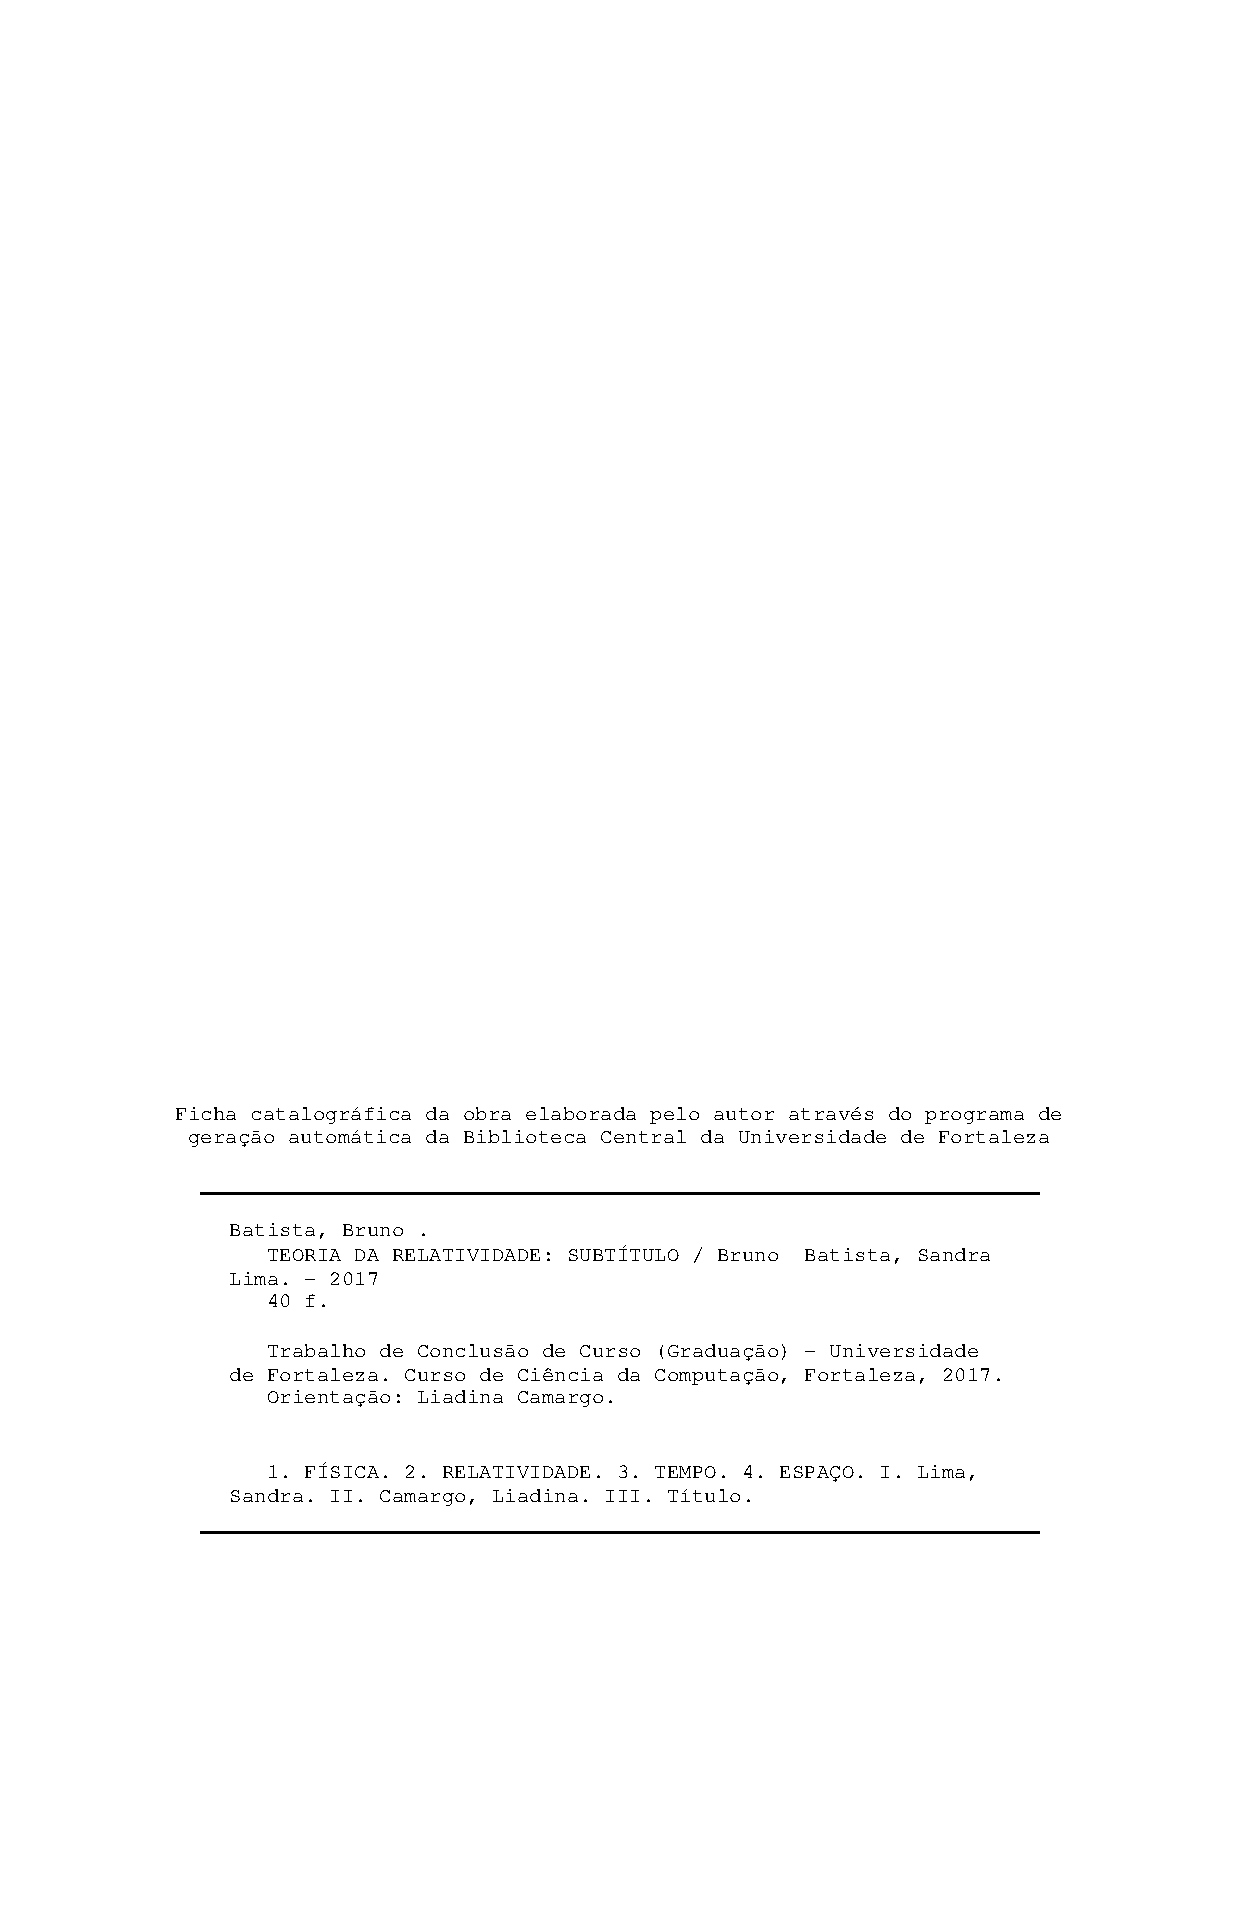
\includepdf{elementos-pre-textuais/folha-aprovacao.pdf} 		%%
	%%					removendo o simbolo de %													%%
	%%			6 - Adicione o simbolo % na linha 	\imprimirfolhadeaprovacao						%%
	%%			7 - Recompile o projeto																%%
	%%																								%%	%%%%%%%%%%%%%%%%%%%%%%%%%%%%%%%%%%%%%%%%%%%%%%%%%%%%%%%%%%%%%%%%%%%%%%%%%%%%%%%%%%%%%%%%%%%%%%%%%%
	
	%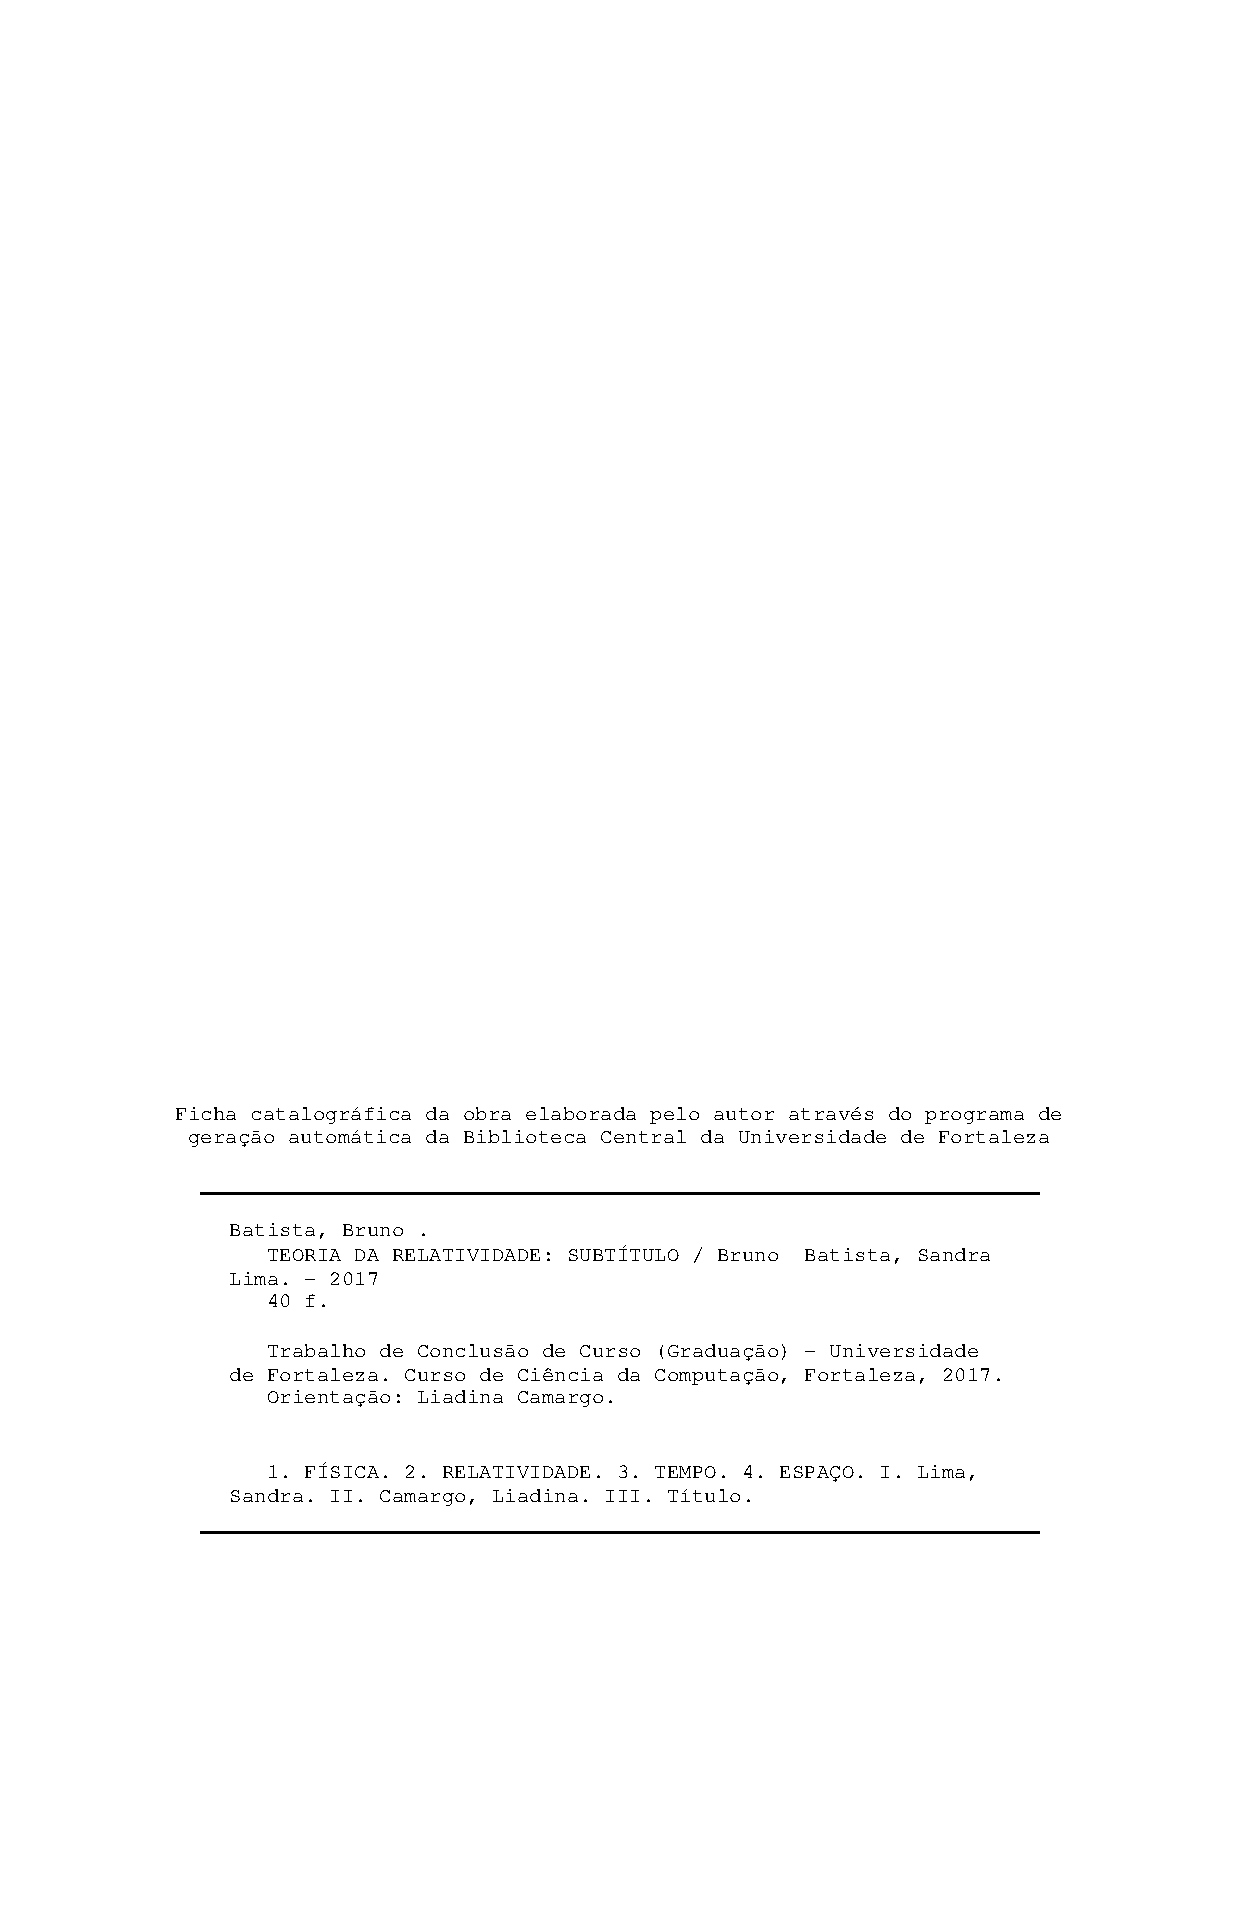
\includepdf{elementos-pre-textuais/folha-aprovacao.pdf}
	\imprimirfolhadeaprovacao
	
	\imprimirdedicatoria{elementos-pre-textuais/dedicatoria}
	\imprimiragradecimentos{elementos-pre-textuais/agradecimentos}
	\imprimirepigrafe{elementos-pre-textuais/epigrafe}
	\imprimirresumo{elementos-pre-textuais/resumo}
	\imprimirabstract{elementos-pre-textuais/abstract}
	\imprimirlistadeilustracoes
	\imprimirlistadetabelas
	\imprimirlistadequadros
	\imprimirlistadealgoritmos
	\imprimirlistadecodigosfonte
	\imprimirlistadeabreviaturasesiglas
	\imprimirlistadesimbolos{elementos-pre-textuais/lista-de-simbolos}
	\imprimirsumario

	%Elementos textuais
	\textual
	\chapter{Introdução}
\label{}
Devido a um problema de analise climáticas de certas regiões de difícil acesso como no nordeste, para monitorar as condições meteorológicas para buscar entender melhor sobre o funcionamento e uso na agricultura. 

Para levantamento de informações sobre as condições climáticas Como temperatura, umidade, pressão e luminosidade é necessário muita observação, prática ,seguir horários e gerenciamentos das atividades, que podem afeta muito nas tomadas de decisões a longo prazo  e também nesse ramo dependem de boas condições climáticas para ter sucesso como fazer plantação, pequenas construções e ate mesmo saber se esta confortável para os trabalhadores exercerem suas atividades.  

Com base desses problemas eu formulei um projeto de sistemas embarcados para desenvolver uma estação meteorológica justamente para registar os fenômenos climáticos e possibilitar um monitoramento das variáveis climáticas.

A estação funciona através de sensores, a coleta e a medição de dados climáticos e auxiliar quem esta buscando a melhorar o seu cultivo. E com bases nesses dados obtidos através dos sensores mostrar a situação climática em um dispositivo portátil sem fio facilitando o monitoramento das atividades  agrária. A partir dessas considerações visa-se responder a seguinte pergunta: Como podemos analisar e monitorar melhor as situações climáticas em qualquer lugar? 

Sobre esse projeto envolve algumas tecnologias de sistemas embarcados, que tem a vital importância para automação e são bastante utilizado  no nosso cotidiano, sendo mais viável para solucionar problemas a longo prazo. O Embarcado a ser utilizado é o ESP32 que tem bom poder de processamento tendo um microcontrolador com 2 núcleos, comunicação WI-FI,  podendo integrar com vários sensores e atuadores e acompanha com vários recursos que torna o uso em Internet das coisas algo bem interessante. 

Nessa tecnologia faz integração com os sensores, que são os periféricos que captam o ambiente e gera a informação para o sistema como temperatura, umidade em forma de sinal e o mesmo gerencia esses periféricos e faz a interface com o dispositivo de saída que nesse caso as afirmações são mostradas na tela do celular.  

Antigamente o sistema embarcados era utilizado apenas para aplicações especificas utilizando codificação de alto nível que o torna complicado para desenvolvimento de algumas soluções, atualmente conta com diversas unidades de processamento e com bom desempenho que suporta diversos equipamentos facilitando o desenvolvimento de vários projetos.  

Enfim é bem interessante desenvolver uma estação meteorológica para auxilias as pessoas que esta começando o seu ramo de negócio agrário, que necessitam de informações captadas usando uma placa  ESP32 interligando com vários sensores e mostrando as variáveis climáticas pelo aplicativo em uma rede sem fio. 




\section{Motivação}
\label{sec:motivacao}

Na falta de recursos e na dificuldade de tomar decisões em monitorar os recursos agrários.

\section{Objetivos}
\label{sec:objetivos}



\subsection{Objetivo Geral}
\label{sec:objetivo-geral}

Objetivo deste trabalho é desenvolver ao longo de analise e pesquisa, uma aplicação que usa os recursos dos sistemas embarcados.            

\subsection{Objetivos Específicos}
\label{sec:objetivos-especificos}



	\begin{alineas}
		\item Elaborar um estudo de caso sobre a aplicação.
		\item Desenvolver a programação e entender o funcionamento de cada tarefa.
		\item Montar o projeto baseado nas pesquisas, interligando com os sensores necessários.
		\item Realizar uma analise, teste e experimentos sobre o funcionamento do projeto.
		\item Apresentar os resultados e desenvolver a comclusão sobre o projeto.
	\end{alineas}
	\chapter{Fundamentação Teórica

	De acordo com Oliveira e ANDRADE (2010), Sistemas embarcados são sistemas computacionais completos e independentes que possui a parte física (Hardware) e Lógica (Software ou Firmware), mais simples que um computador de propósito geral (Desktops), encarregados de executar apenas uma função determinada - tarefas pré-determinadas, com requisitos específicos, na qual executam geralmente repetidas vezes. Por serem muito simples, muitas vezes esses sistemas não têm flexibilidade (de software e de hardware) que lhes permita fazer outras tarefas quaisquer que não sejam aquelas para as quais foram desenhados e desenvolvidos.
Um grande responsável pela expansão do uso e aplicação dos sistemas embarcados foi a utilização do microcontrolador, pelo seu baixo custo, versatilidade e tamanho reduzido. Muitos microcontroladores podem ser conectados a dispositivos analógicos, permitindo o uso de sensores diversos. Isso permite a criação de dispositivos simples, que monitoram temperatura, umidade, entre outros fatores, executando ações predefinidas em caso de mudanças.
Em geral os sistemas embarcados possuem uma capacidade de processamento reduzida em comparação com computadores desktops. Ao invés de utilizar microprocessadores, os desenvolvedores preferem utilizar microcontroladores, pois estes já possuem diversos periféricos integrados no mesmo chip.V850, FR-V Outra diferença é a variedade de arquiteturas disponíveis tais como ARM, MIPS, Coldfire/68k, PowerPC, x86, PIC, 8051, Atmel AVR, Renesas H8, SH, M32R, Z80 e Z8.
Os sistemas embarcados comunicam-se com o meio externo através de periféricos. Estes periféricos podem ser combinados com o processador (como no caso dos sistemas microcontrolados) ou associados no sistema.
Entre os periféricos mais comum temos:
	Entrada de dados através de teclas (geralmente através de teclados feitos com varredura matricial)
Leds
	Displays de LCD (sendo os mais comuns os alfanuméricos por exemplo o HD44780)
Interface serial - (Por exemplo RS 232, I2C)
Universal Serial Bus - (USB)
TCP/IP

 

 

Hardware 
Graças a tecnologia baseada em transistores é possível miniaturizar componentes como os circuitos integrados, processadores e seus periféricos com baixo custo através de encapsulamento permitiu ter uma variedade de dispositivos para uma determinada aplicações e aperfeiçoa-la assim como os conversores analógico- digital (AD) capaz de digitalizar toda a informação em apenas uma fração de tempo.  Possui na sua arquitetura: Unidade Central de Processamento composto por unidade Logica e aritmética, Unidade de controle, Sistema de memória composto por memória de acesso aleatório e de Armazenamento e Sistemas de Entrada e saída interligados por meios de barramentos.
Firmware
É um tipo de Software Embarcado que controla o Hardware usando linguagens de baixo nível (Linguagem de máquina). Ele possui os principais componentes: Sistema básico de entrada e saída (BIOS) BASIC IMPUT OUTPUT SYSTEM serve parar inicializar o sistema, checar os dispositivos e carregar o Sistema Operacional (SO); SETUP responsável por alterar os parâmetros da memória de configuração (CMOS) que é usada para gravar as configurações do SETUP em uma pequena área de memória volátil alimentado por uma bateria. Podendo operar em tempo real onde determinadas tarefas tem o seu prazo compatíveis com a ocorrência dos eventos.
Controller Area Network (CAN)
Baseada em aplicações em tempo real um meio para transmissões de redes e controla o fluxo e propagação de mensagens sendo necessario um cotrole rígido de erro para que haja eficácia no recebimento de mensagens.
Godoy et al; 2010. Afirma que O CAN (Bosch, 2006) é um protocolo de comunicação digital serial e não determinístico, onde a comunicação de dados é baseada em mensagens formadas por quadros de bits com determinada função. Entre esses quadros de bits, existe o campo identificador (identifier ID) que caracteriza e define a prioridade de cada mensagem. O valor do identificador de uma mensagem em uma rede CAN é exclusivo e quanto mais baixo seu valor, maior será a prioridade da mensagem. Os sinais elétricos digitais do CAN são representados pelo nível recessivo (nível lógico 1) e nível dominante (nível lógico 0), sendo eles sinais diferenciais entre os dois fios da rede.(GODOY et al; 2010)
}
\label{cap:fundamentacao-teorica}



\section{Fundamentação Teórica A}

	
	\begin{figure}[h!]
		\centering
		\Caption{\label{fig:exemplo-2} Diagrama básico de um sistema embarcado dotado de um microcontrolador monitorando o ambiente.}	
		\UNIFORfig{}{
			\fbox{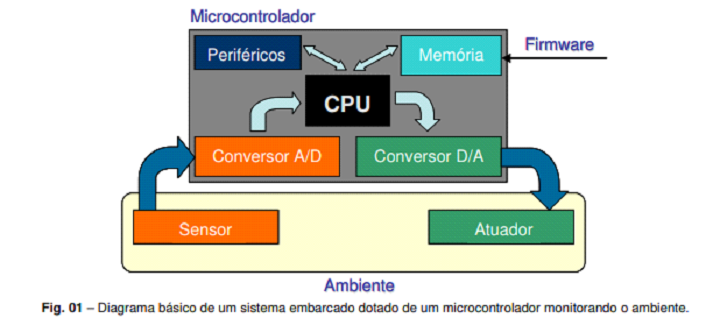
\includegraphics[width=14cm]{figuras/fig01}}
		}{
			\Fonte{Elaborado pelo autor}
		}
		
	\end{figure}
	
		\begin{figure}[h!]
		\centering
		\Caption{\label{fig:exemplo-3} Logica de um sistema embarcado usando um microprocessador como unidade de processamento.}	
		\UNIFORfig{}{
			\fbox{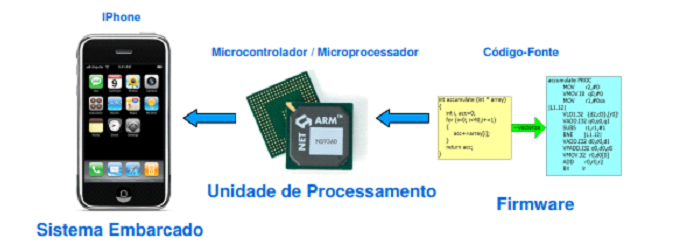
\includegraphics[width=14cm]{figuras/fig02}}
		}{
			\Fonte{Elaborado pelo autor}
		}	
	\end{figure}
	



\section{Fundamentação Teórica B}
\label{sec:fundamentacao-teorica-b}

Integer non lacinia magna. Aenean tempor lorem tellus, non sodales nisl commodo ut. Proin mattis placerat risus sit amet laoreet. Praesent sapien arcu, maximus ac fringilla efficitur, vulputate faucibus sem. Donec aliquet velit eros, sit amet elementum dolor pharetra eget. Integer eget mattis libero. Praesent ex velit, pulvinar at massa vel, fermentum dictum mauris. Ut feugiat accumsan augue, et ultrices ipsum euismod vitae

	\begin{figure}[h!]
		\centering
		\Caption{\label{fig:exemplo-2} Maecenas luctus augue odio, sed tincidunt nunc posuere nec}	
		\UNIFORfig{}{
			\fbox{
\includegraphics[width=8cm]{figuras/figura-2}}
		}{
			\Fonte{Elaborado pelo autor}			
		}	
	\end{figure}

Nunc ac pretium dui. Mauris aliquam dapibus nulla ac mattis. Aenean non tortor volutpat, varius lectus vitae, accumsan nibh. Cras pretium vestibulum enim, id ullamcorper tortor ultrices non. Integer sodales viverra faucibus. Curabitur at dui lacinia, rhoncus lacus at, blandit metus. Integer scelerisque non enim quis ornare.

\lipsum[13]

	\begin{table}[h!]	
		\centering
		\Caption{\label{tab:exemplo-1} Duis faucibus, enim quis tincidunt pellentesque, nisl leo varius nulla, vitae tempus dui mauris ac ante purus lorem}		
		\UNIFORtab{}{
			\begin{tabular}{cll}
				\toprule
				Ranking & Exon Coverage & Splice Site Support \\
				\midrule \midrule
				E1 & Complete coverage by a single transcript & Both splice sites\\
				E2 & Complete coverage by more than a single transcript & Both splice sites\\
				E3 & Partial coverage & Both splice sites\\
				E4 & Partial coverage & One splice site\\
				E5 & Complete or partial coverage & No splice sites\\
				E6 & No coverage & No splice sites\\
				\bottomrule
			\end{tabular}
		}{
		\Fonte{Elaborado pelo autor}
	}
	\end{table}

Evidentemente, a contínua expansão de nossa atividade obstaculiza a apreciação da importância das formas de ação. Por outro lado, o comprometimento entre as equipes nos obriga à análise dos métodos utilizados na avaliação de resultados. Acima de tudo, é fundamental ressaltar que a necessidade de renovação processual talvez venha a ressaltar a relatividade das novas proposições. 

          Do mesmo modo, a constante divulgação das informações auxilia a preparação e a composição do retorno esperado a longo prazo. No entanto, não podemos esquecer que a hegemonia do ambiente político garante a contribuição de um grupo importante na determinação das diversas correntes de pensamento. A certificação de metodologias que nos auxiliam a lidar com o desenvolvimento contínuo de distintas formas de atuação assume importantes posições no estabelecimento dos relacionamentos verticais entre as hierarquias. 

          Podemos já vislumbrar o modo pelo qual a estrutura atual da organização exige a precisão e a definição dos modos de operação convencionais. As experiências acumuladas demonstram que a execução dos pontos do programa prepara-nos para enfrentar situações atípicas decorrentes das condições inegavelmente apropriadas. Caros amigos, a consulta aos diversos militantes afeta positivamente a correta previsão das condições financeiras e administrativas exigidas. Desta maneira, a competitividade nas transações comerciais é uma das consequências de todos os recursos funcionais envolvidos. 

          Não obstante, a expansão dos mercados mundiais pode nos levar a considerar a reestruturação das diretrizes de desenvolvimento para o futuro. Todavia, a mobilidade dos capitais internacionais cumpre um papel essencial na formulação dos paradigmas corporativos. O cuidado em identificar pontos críticos no novo modelo estrutural aqui preconizado ainda não demonstrou convincentemente que vai participar na mudança do processo de comunicação como um todo. É importante questionar o quanto a adoção de políticas descentralizadoras deve passar por modificações independentemente das direções preferenciais no sentido do progresso. Pensando mais a longo prazo, o fenômeno da Internet causa impacto indireto na reavaliação do investimento em reciclagem técnica. 

	\begin{figure}[h!]
		\centering
		\Caption{\label{fig:exemplo-3} Ut posuere, ex quis sagittis auctor, magna massa euismod felis}	
		\UNIFORfig{}{
			\fbox{
\includegraphics[width=8cm]{figuras/figura-2}}
		}{
		\Fonte{Elaborado pelo autor}			
	}	
	\end{figure}

\lipsum[14]

	\begin{table}[h!]	
		\centering
		\Caption{\label{tab:exemplo-2} Etiam molestie, nulla a egestas aliquet, velit augue congue metus}		
		\UNIFORtab{}{
			\begin{tabular}{ccll}
				\toprule
				Quisque & pharetra & tempus & vulputate \\
				\midrule \midrule
				E1 & Complete coverage by a single transcript & Both splice sites\\
				E2 & Complete coverage by more than a single transcript & Both splice sites\\
				E3 & Partial coverage & Both splice sites & Both \\
				E4 & Partial coverage & One splice site & Both \\
				E5 & Complete or partial coverage & No splice sites & Both\\
				E6 & No coverage & No splice sites\\
				\bottomrule
			\end{tabular}
		}{
		\Fonte{Elaborado pelo autor}
	}
	\end{table}
	
Duis faucibus, enim quis tincidunt pellentesque, nisl leo varius nulla, vitae tempus dui mauris ac ante. Quisque purus lorem, pharetra sit amet lobortis eu, vehicula vitae purus.
\acrlong{DATASUS},\acrlong{DNV},\acrlong{DO},\acrlong{ESF},\acrlong{IBGE},\acrlong{MFC},\acrlong{MI},\acrlong{MS},\acrlong{NV},\acrlong{ODM},\acrlong{OI},\acrlong{OMS},\acrlong{ONU},\acrlong{PNI},\acrlong{PSF},\acrlong{RIPSA},\acrlong{RN},\acrlong{SIM},\acrlong{SINASC},\acrlong{SUS},\acrlong{TMI},\acrlong{TMMFC}

\begin{alineascomponto}
	\item Integer non lacinia magna. Aenean tempor lorem tellus, non sodales nisl commodo ut
	\item Proin mattis placerat risus sit amet laoreet. Praesent sapien arcu, maximus ac fringilla efficitur, vulputate faucibus sem. Donec aliquet velit eros, sit amet elementum dolor pharetra eget
	\item Integer eget mattis libero. Praesent ex velit, pulvinar at massa vel, fermentum dictum mauris. Ut feugiat accumsan augue, et ultrices ipsum euismod vitae
	\begin{subalineascomponto}
		\item Integer non lacinia magna. Aenean tempor lorem tellus, non sodales nisl commodo ut
		\item Proin mattis placerat risus sit amet laoreet.
	\end{subalineascomponto}
\end{alineascomponto}
	\chapter{Trabalhos Relacionados}
\label{cap:trabalhos-relacionados}

Integer non lacinia magna. Aenean tempor lorem tellus, non sodales nisl commodo ut. Proin mattis placerat risus sit amet laoreet. Praesent sapien arcu, maximus ac fringilla efficitur, vulputate faucibus sem. Donec aliquet velit eros, sit amet elementum dolor pharetra eget. Integer eget mattis libero

\section{Trabalho Relacionado A}
\label{sec:trabalho-relacionado-a}

\lipsum[10]

	\begin{figure}[h!]
		\centering
		\Caption{\label{fig:exemplo-1} Lorem ipsum dolor sit amet, consectetur adipiscing elit. Suspendisse commodo lectus et augue elementum varius.}	
		\UNIFORfig{}{
			\fbox{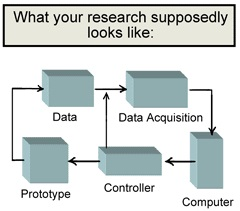
\includegraphics[width=8cm]{figuras/figura-1}}
		}{
			\Fonte{Elaborado pelo autor}
		}	
	\end{figure}
	
\lipsum[11]

\section{Trabalho Relacionado B}
\label{sec:trabalho-relacionado-b}

Integer non lacinia magna. Aenean tempor lorem tellus, non sodales nisl commodo ut. Proin mattis placerat risus sit amet laoreet. Praesent sapien arcu, maximus ac fringilla efficitur, vulputate faucibus sem. Donec aliquet velit eros, sit amet elementum dolor pharetra eget. Integer eget mattis libero. Praesent ex velit, pulvinar at massa vel, fermentum dictum mauris. Ut feugiat accumsan augue, et ultrices ipsum euismod vitae

	\begin{figure}[h!]
		\centering
		\Caption{\label{fig:exemplo-2} Maecenas luctus augue odio, sed tincidunt nunc posuere nec}	
		\UNIFORfig{}{
			\fbox{
\includegraphics[width=8cm]{figuras/figura-2}}
		}{
			\Fonte{Elaborado pelo autor}			
		}	
	\end{figure}

Nunc ac pretium dui. Mauris aliquam dapibus nulla ac mattis. Aenean non tortor volutpat, varius lectus vitae, accumsan nibh. Cras pretium vestibulum enim, id ullamcorper tortor ultrices non. Integer sodales viverra faucibus. Curabitur at dui lacinia, rhoncus lacus at, blandit metus. Integer scelerisque non enim quis ornare.

	\begin{quadro}[h!]	
		\centering
		\Caption{\label{qua:exemplo-1} Praesent ex velit, pulvinar at massa vel, fermentum dictum mauris. Ut feugiat accumsan augue}		
		\UNIFORqua{}{
			\begin{tabular}{|c|c|l|l|}
				\hline
				Quisque & pharetra & tempus & vulputate \\
				\hline
				E1 & Complete coverage by a single transcript & Both  & Complete\\
				\hline
				E2 & Complete coverage by more than & Both splice sites & Complete\\
				\hline
				E3 & Partial coverage & Both splice sites & Both \\				
				\hline
			\end{tabular}
		}{
			\Fonte{Elaborado pelo autor}
		}
	\end{quadro}
	
\lipsum[20]

	
	\begin{quadro}[h!]	
		\centering
		\Caption{\label{qua:exemplo-2} Duis faucibus, enim quis tincidunt pellentesque}		
		\UNIFORqua{}{
			\begin{tabular}{|c|c|}
				\hline
				Quisque & pharetra \\
				\hline
				E1 & Complete coverage by a single transcript \\
				\hline
				E2 & Complete coverage by more than \\
				\hline
				E3 & Partial coverage \\
				\hline
				E4 & Partial coverage \\
				\hline
				E5 & Partial coverage \\
				\hline
				E6 & Partial coverage \\
				\hline
				E7 & Partial coverage \\
				\hline
			\end{tabular}
		}{
			\Fonte{Elaborado pelo autor}
		}
	\end{quadro}

\lipsum[21]

Integer non lacinia magna. Aenean tempor lorem tellus, non sodales nisl commodo ut. Proin mattis placerat risus sit amet laoreet. Praesent sapien arcu, maximus ac fringilla efficitur, vulputate faucibus sem. Donec aliquet velit eros, sit amet elementum dolor pharetra eget. Integer eget mattis libero.
\Gls{ambiguidade}
\Gls{braile}
\Gls{coerencia}
\Gls{dialetos}
\Gls{elipse}
\Gls{locucao-adjetiva}
\Gls{modificadores}
\Gls{paronimos}
\Gls{sintese}
\Gls{borboleta}
	\chapter{Metodologia}
\label{chap:metodologia}

\lipsum[2]
\lipsum[12]

O autor \cite{lamport1986latex} e \cite{Maia2011} \lipsum[2] 

\begin{table}[h!]
	\Caption{\label{tabela-ibge} Um Exemplo de tabela alinhada que pode ser longa ou curta, conforme padrão IBGE}%
	\IBGEtab{}{%
		\begin{tabular}{ccc}
			\toprule
			Nome & Nascimento & Documento \\
			\midrule \midrule
			Maria da Silva & 11/11/1111 & 111.111.111-11 \\
			Maria da Silva & 11/11/1111 & 111.111.111-11 \\
			Maria da Silva & 11/11/1111 & 111.111.111-11 \\
			\bottomrule
		\end{tabular}%
	}{%
	\Fonte{Produzido pelos autores}%
	\Nota{Esta é uma nota, que diz que os dados são baseados na
		regressão linear.}%
	\Nota[Anotações]{Uma anotação adicional, seguida de várias outras.}%
}
\end{table}

\cite{Huetal2000} \lipsum[2] 

\section{Exemplo de Algoritmos e Figuras}
\label{sec:exemplo-de-algoritmos-e-figuras}

\lipsum[2]

\begin{algorithm}[h!]
	\SetSpacedAlgorithm
	\caption{\label{exemplo-de-algoritmo}Como escrever algoritmos no \LaTeX2e}
	\Entrada{o proprio texto}
	\Saida{como escrever algoritmos com \LaTeX2e }
	\Inicio{
		inicializa\c{c}\~ao\;
		\Repita{fim do texto}{
			leia o atual\;
			\Se{entendeu}{
				vá para o próximo\;
				próximo se torna o atual\;}
			\Senao{volte ao início da seção\;}
		}
	}	
\end{algorithm}

\lipsum[2]
%\begin{algorithm}[H]
%	\Entrada{o proprio texto}
%	\Saida{como escrever algoritmos com \LaTeX2e }
%	\Inicio{
%		inicializa\c{c}\~ao\;
%		\Repita{fim do texto}{
%			leia o atual\;
%			\Se{entendeu}{
%				vá para o próximo\;
%				próximo se torna o atual\;}
%			\Senao{volte ao início da seção\;}
%		}
%	}
%	\caption{Exemplo de Algoritmo Versao 02}
%\end{algorithm}

%\begin{algorithm}
%	\begin{algorithmic}
%	\Entrada{o proprio texto}
%	\Saida{como escrever algoritmos com \LaTeX2e }	
%	\end{algorithmic}
%\end{algorithm}

Exemplo de alíneas com números:

\begin{alineascomnumero}
	\item Lorem ipsum dolor sit amet, consectetur adipiscing elit. Nunc dictum sed tortor nec viverra.
	\item Praesent vitae nulla varius, pulvinar quam at, dapibus nisi. Aenean in commodo tellus. Mauris molestie est sed justo malesuada, quis feugiat tellus venenatis.
	\item Praesent quis erat eleifend, lacinia turpis in, tristique tellus. Nunc dictum sed tortor nec viverra.
	\item Mauris facilisis odio eu ornare tempor. Nunc dictum sed tortor nec viverra.
	\item Curabitur convallis odio at eros consequat pretium.
\end{alineascomnumero}

\lipsum[12]

\begin{table}[h!]	
	\centering
	\Caption{\label{tab:internal}Internal exon scores}	
	\IBGEtab{}{
		\begin{tabular}{cll}
			\toprule
			Ranking & Exon Coverage & Splice Site Support\\
			\midrule \midrule
			E1 & Complete coverage by a single transcript & Both splice sites\\
			E2 & Complete coverage by more than a single transcript & Both splice sites\\
			E3 & Partial coverage & Both splice sites\\
			E4 & Partial coverage & One splice site\\
			E5 & Complete or partial coverage & No splice sites\\
			E6 & No coverage & No splice sites\\
			\bottomrule
		\end{tabular}
	}{
	\Fonte{os autores}
}
\end{table}

\lipsum[2] Referenciando a \autoref{tab:internal} \lipsum[2]

\index{figuras}Figuras podem ser criadas diretamente em LaTeX,
como o exemplo da \ref{fig-grafico-1}.

\begin{figure}[h!]
	\centering
	\Caption{\label{fig-grafico-1}Produção anual das dissertações de mestrado e teses de doutorado entre os anos de 1990 e 2008}		
	\IBGEtab{}{
		\fbox{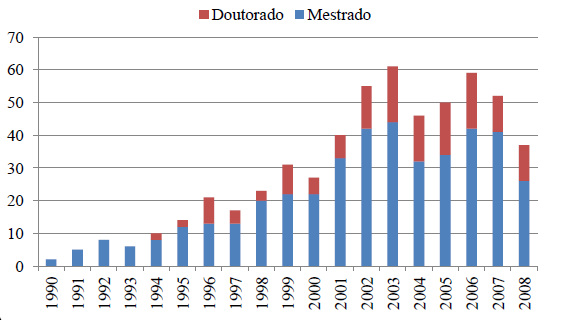
\includegraphics[scale=0.5]{figuras/figura-3}}
	}{
	\Fonte{os autores}
}
\end{figure}

Ou então figuras podem ser incorporadas de arquivos externos, como é o caso da \autoref{fig-grafico-1}. Se a figura que ser incluída se tratar de um diagrama, um gráfico ou uma ilustração que você mesmo produza, priorize o uso de imagens vetoriais no formato PDF. Com isso, o tamanho do arquivo final do trabalho será menor, e as imagens terão uma apresentação melhor, principalmente quando impressas, uma vez que imagens vetorias são perfeitamente escaláveis para qualquer dimensão. Nesse caso, se for utilizar o Microsoft Excel para produzir gráficos, ou o Microsoft Word para produzir ilustrações, exporte-os como PDF e os incorpore ao documento conforme o exemplo abaixo. No entanto, para manter a coerência no uso de software livre (já que você está usando LaTeX e abnTeX),  teste a ferramenta InkScape\index{InkScape}. ao CorelDraw\index{CorelDraw} ou ao Adobe Illustrator\index{Adobe! Illustrator}.  De todo modo, caso não seja possível  utilizar arquivos de imagens como PDF, utilize qualquer outro formato, como JPEG, GIF, BMP, etc.  Nesse caso, você pode tentar aprimorar as imagens incorporadas com o software livre \index{Gimp}Gimp. Ele é uma alternativa livre ao Adobe Photoshop\index{Adobe! Photoshop}.

\section{Usando Fórmulas Matemáticas}

\lipsum[2]

	\begin{equation}
		\begin{aligned}
			x = a_0 + \cfrac{1}{a_1
				+ \cfrac{1}{a_2
					+ \cfrac{1}{a_3 + \cfrac{1}{a_4} } } }
		\end{aligned}
	\end{equation}

\lipsum[3]

	\begin{equation}
		\begin{aligned}
			k_{n+1} = n^2 + k_n^2 - k_{n-1}
		\end{aligned}
	\end{equation}

\lipsum[4]

	\begin{equation}
		\begin{aligned}
			\cos (2\theta) = \cos^2 \theta - \sin^2 \theta
		\end{aligned}
	\end{equation}
	
\lipsum[5]

	\begin{equation}
		\begin{aligned}
			A_{m,n} =
			\begin{pmatrix}
			a_{1,1} & a_{1,2} & \cdots & a_{1,n} \\
			a_{2,1} & a_{2,2} & \cdots & a_{2,n} \\
			\vdots  & \vdots  & \ddots & \vdots  \\
			a_{m,1} & a_{m,2} & \cdots & a_{m,n}
			\end{pmatrix}
		\end{aligned}
	\end{equation}

\lipsum[6]

	\begin{equation}
		\begin{aligned}
			f(n) = \left\{ 
			\begin{array}{l l}
			n/2 & \quad \text{if $n$ is even}\\
			-(n+1)/2 & \quad \text{if $n$ is odd}
			\end{array} \right.
		\end{aligned}
	\end{equation}
	
\lipsum[7]

\section{Usando Algoritmos}

\lipsum[8]

\begin{algorithm}[h!]
	\SetSpacedAlgorithm
	\caption{\label{alg:algoritmo_de_colonica_de_formigas}Algoritmo de Otimização por Colônia de Formiga}
	\Entrada{Entrada do Algoritmo}
	\Saida{Saida do Algoritmo}
	\Inicio{
		Atribua os valores dos parâmetros\;
		Inicialize as trilhas de feromônios\;
		\Enqto{não atingir o critério de parada}{
			\Para{cada formiga}{
				Construa as Soluções\;
			}
			Aplique Busca Local (Opcional)\;
			Atualize o Feromônio\;
		}	
	}		
\end{algorithm}

\lipsum[9]

\section{Usando Código-fonte}

\lipsum[10]

\lstinputlisting[language=C++,caption={Hello World em C++}]{figuras/main.cpp}

\lipsum[11]

\begin{lstlisting}[language=Java,caption={Hello World em Java}]
public class HelloWorld {
	public static void main(String[] args) {
		System.out.println("Hello World!");
	}
}
\end{lstlisting}

\lipsum[11]

\section{Usando Teoremas, Proposições, etc}

Lorem ipsum dolor sit amet, consectetur adipiscing elit. Nunc dictum sed tortor nec viverra. consectetur adipiscing elit. Nunc dictum sed tortor nec viverra.

\begin{teo}[Pitágoras]
	Em todo triângulo retângulo o quadrado do comprimento da
	hipotenusa é igual a soma dos quadrados dos comprimentos dos catetos.
\end{teo}


Lorem ipsum dolor sit amet, consectetur adipiscing elit. Nunc dictum sed tortor nec viverra. consectetur adipiscing elit. Nunc dictum sed tortor nec viverra.

\begin{teo}[Fermat]
	Não existem inteiros $n > 2$, e $x, y, z$ tais que $x^n + y^n = z$
\end{teo}

Lorem ipsum dolor sit amet, consectetur adipiscing elit. Nunc dictum sed tortor nec viverra. consectetur adipiscing elit. Nunc dictum sed tortor nec viverra.

\begin{prop}
	Para demonstrar o Teorema de Pitágoras...
\end{prop}

Lorem ipsum dolor sit amet, consectetur adipiscing elit. Nunc dictum sed tortor nec viverra. consectetur adipiscing elit. Nunc dictum sed tortor nec viverra.

\begin{exem}
	Este é um exemplo do uso do ambiente exe definido acima.
\end{exem}

Lorem ipsum dolor sit amet, consectetur adipiscing elit. Nunc dictum sed tortor nec viverra. consectetur adipiscing elit. Nunc dictum sed tortor nec viverra.

\begin{xdefinicao}
	Definimos o produto de ...
\end{xdefinicao}

Lorem ipsum dolor sit amet, consectetur adipiscing elit. Nunc dictum sed tortor nec viverra. consectetur adipiscing elit. Nunc dictum sed tortor nec viverra.

\section{Usando Questões}


Lorem ipsum dolor sit amet, consectetur adipiscing elit. Nunc dictum sed tortor nec viverra. consectetur adipiscing elit. Nunc dictum sed tortor nec viverra.

\begin{questao}
	\item Esta é a primeira questão com alguns itens:
		\begin{enumerate}
			\item Este é o primeiro item
			\item Segundo item
		\end{enumerate}
	\item Esta é a segunda questão:
		\begin{enumerate}
			\item Este é o primeiro item
			\item Segundo item
		\end{enumerate}
	\item Lorem ipsum dolor sit amet, consectetur adipiscing elit. Nunc dictum sed tortor nec viverra. consectetur adipiscing elit. Nunc dictum sed tortor nec viverra.
		\begin{enumerate}
			\item consectetur
			\item adipiscing
			\item Nunc
			\item dictum
		\end{enumerate}
\end{questao}

\section{Citações}

\subsection{Documentos com três autores}

Quando houver três autores na citação, apresentam se os três, separados por ponto e vírgula, caso estes estejam após o texto. Se os autores estiverem incluídos no texto, devem ser separados por vírgula e pela conjunção "e".

\citeautoronline{tresautores}

\cite{tresautores}

\subsection{Documentos com mais de três autores}
Havendo mais de três autores, indica-se o primeiro seguido da expressão \textit{et al.} (do latim \textit{et alli}, que significa e outros), do ano e da página.

\citeautoronline{quatroautores}

\cite{quatroautores}

\subsection{Documentos de vários autores}

Havendo    citações    indiretas de    diversos    documentos    de    vários    autores, mencionados  simultaneamente e  que  expressam  a  mesma  ideia,  separam-se  os  autores  por ponto e vírgula, em ordem alfabética.

\cite{tresautores, quatroautores}

\section{Notas de Rodap\'{e}}

Deve-se utilizar o sistema autor-data para as  citações no texto e o numérico para notas explicativas\footnote{Veja - se como exemplo desse tipo de abordagem o estudo de Netzer (1976)}. As notas de rodapé podem e devem ser alinhadas, a partir da segunda linha da mesma nota, abaixo da primeira letra da primeira palavra, de forma a destacar o expoente \footnote{Encontramos  esse  tipo  de  perspectiva  na  2ª  parte  do  verbete  referido  na  nota  anterior,  em  grande  parte  do estudo de Rahner (1962).} e sem espaço entre elas e com fonte menor (tamanho 10).


	\chapter{Resultados esperados}
\label{chap:resultados}
O projeto funcionando com o módulo ESP32 recebendo os dados através dos sensores interligados captando o ambiente, processando esses dados e enviando as informações pelo sinal wi-fi para que os aparelhos que usam o endereço IP mostrasse os resultados ao usuário.


	\chapter{Conclusões e Trabalhos Futuros}
\label{chap:conclusoes-e-trabalhos-futuros}

\lipsum[2]
\lipsum[34]

\section{Contribuições do Trabalho}
\label{sec:contribuicoes-do-trabalho}

\lipsum[3]

\section{Limitações}
\label{sec:limitacoes}

\lipsum[4]

\section{Trabalhos Futuros}
\label{sec:trabalhos-futuros}

\lipsum[5]






	%Elementos pós-textuais
	\bibliography{elementos-pos-textuais/referencias}
	\imprimirglossario
	\imprimirapendices
		% Adicione aqui os apendices do seu trabalho
		\apendice{Lorem Ipsum}
\label{ap:lorem-ipsum}

\lipsum[1]
		\apendice{Modelo de Capa}
\label{ap:modelo-de-capa}



%		\apendice{Termo de Fiel Depositário}
\label{ap:termo-de-fiel-depositario}

\noindent \textbf{Pesquisa:} ANÁLISE DA MORTALIDADE INFANTIL COM MALFORMAÇÕES CONGÊNITAS.

\noindent Pelo presente instrumento que atende às exigências legais, a Sra. Maria Consuelo Martins Saraiva, ``fiel depositário'' com o cargo de Secretária Municipal de Saúde de Iracema, após ter tomado conhecimento do protocolo de pesquisa intitulado: ANÁLISE DA MORTALIDADE INFANTIL COM MALFORMAÇÕES CONGÊNITAS. Analisando a repercussão desse estudo no contexto da saúde pública e epidemiologia, autoriza Karla Maria da Silva Lima, enfermeira, aluna do Curso de Mestrado Acadêmico em Enfermagem da Universidade Estadual do Ceará (UECE), sob orientação do Prof. Dr. José Maria de Castro, da UECE, ter acesso aos bancos de dados do Sistema de Informação sobre Nascidos Vivos e do Sistema de Informação sobre Mortalidade da Secretaria Municipal de Saúde de Iracema, objeto deste estudo, e que se encontram sob sua total responsabilidade. Fica claro que o Fiel Depositário pode a qualquer momento retirar sua AUTORIZAÇÃO e ciente de que todas as informações prestadas tornar-se-ão confidenciais e guardadas por força de sigilo profissional, assegurando que os dados obtidos da pesquisa serão somente utilizados para estudo.
	\imprimiranexos
		% Adicione aqui os anexos do seu trabalho
		\anexo{Exemplo de Anexo}
\label{an:exemplo-de-anexo}

\lipsum[13]
		\anexo{Titulo}
\label{an:Titulo}

	\imprimirindice

\end{document}
